% ITEX root = ../Thesis.tex

Filtering and wrangling the data resulted in 305 different unique sub-data sets being produced, saving the data frames of time and common logarithm of the population, and the respective unique species ID in \textit{.rda} files. The plots to show the trend in population over time has time along the x-axis and Abundance along the y-axis. Plots revealed an inconsistent distribution of the data set, some sigmoidal, log distributed or completely random.  All starting parameter values were generated for 298 of the 305 data sets and any negative growth rate slopes $r_{max}$ was set to NA.

Optimal parameter values were obtained for most of the unique data sets. The Buchanan model had 105 fits, Baranyi model had 218 fits, Gompertz model had 211 fits and finally the Logistic model had the most with 241 fits. The models fit approximately 80% of the data. Of the 305 data sets, 243 total model fittings were successfully produced. From the 243 fittings, the best model was the one with the lowest AIC value. The distribution of best fit was uneven among the four models, as majority of the relative best fits was by the Gompertz model, with 99 of the 243, while the next best fit was the Baranyi model with 66, and Logistic and Buchanan with 51 and 27 respectively.
\begin{figure*}[h!]
    \centering
    \begin{subfigure}[h]{0.4\textwidth}
        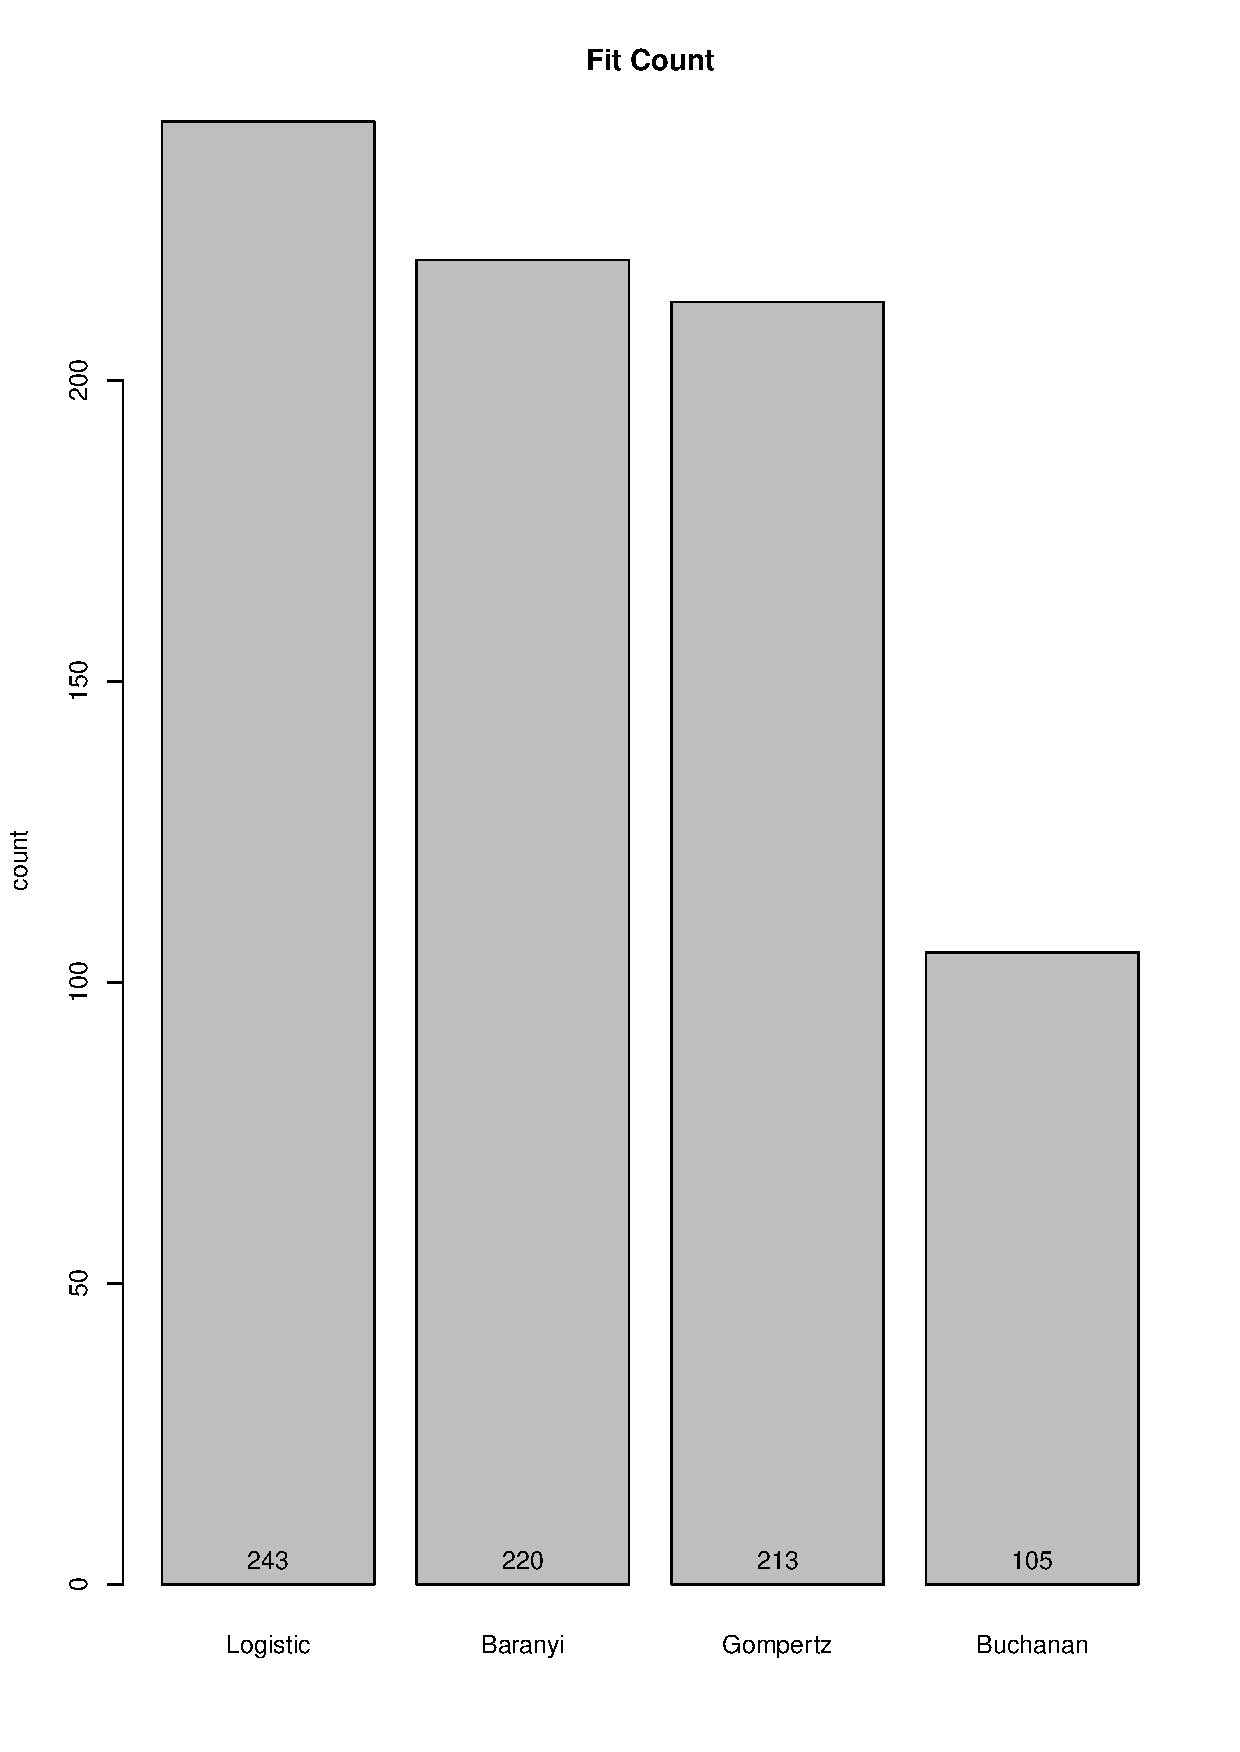
\includegraphics[width=\textwidth]{../Results/Fit_count.pdf}
        \caption{Figure 2.1: Barplot of the number of successful fits for each model}
        \label{fig:Fit Count}
    \end{subfigure}
    \hfill
    \begin{subfigure}[h]{0.4\textwidth}
        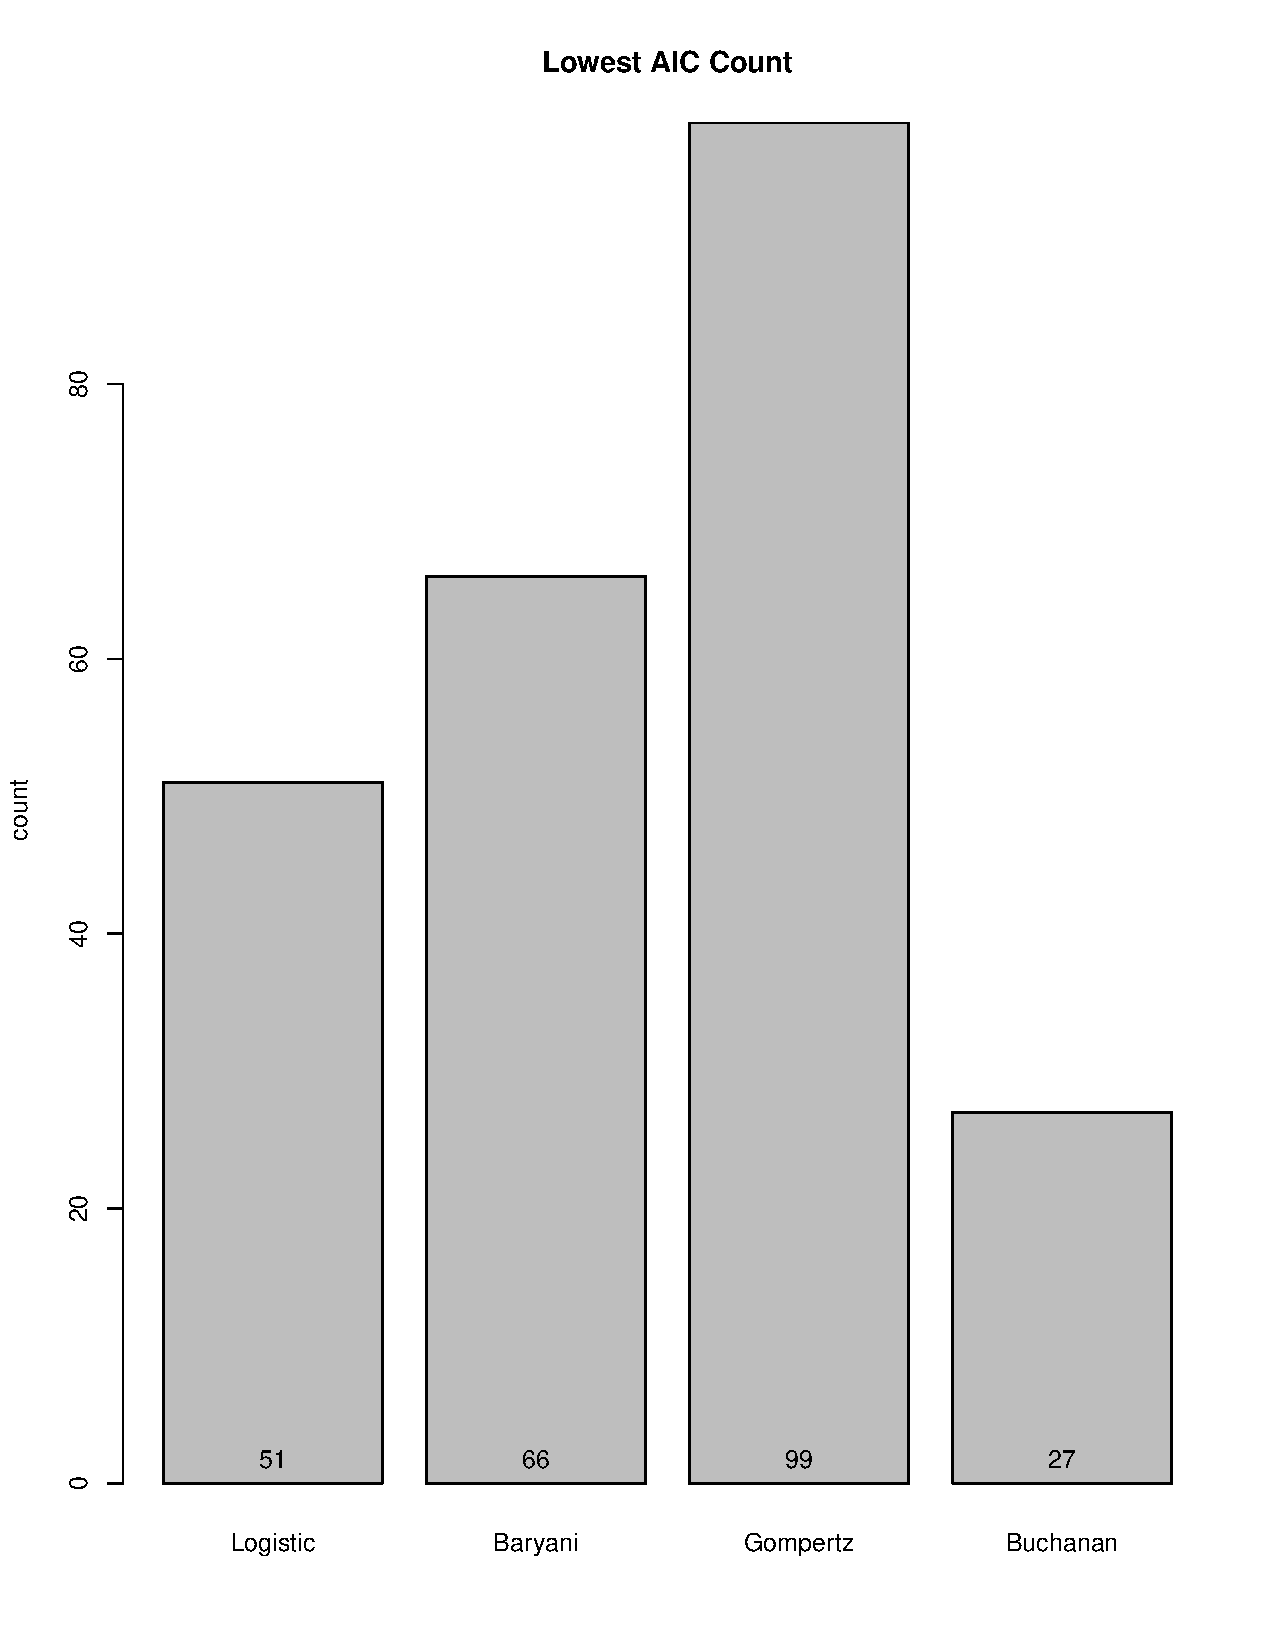
\includegraphics[scale=0.35]{../Results/bestfit_barplot.pdf}
        \caption{Figure 2.2: Barplot showing count of lowest AIC scores for each of the models tested on the data}
        \label{fig:AIC count}
    \end{subfigure}
\end{figure*}

In the additional investigation from the paper, conceptual temperature recordings existed for five of the species from the published data. These five species and their data were subsetted, and linear regression analysis was carried out. The plots include two lines, the linear regression line, and the formula \begin{equation*}\sqrt{r}=b(T-T_0)\end{equation*}\cite{ratkowsky1982relationship}. Temperature along the x-axis was plotted against $\sqrt{r}$ on the y-axis as recommended by \textit{Ratkowsky et al.} Visualisation of the results shows that the growth rate is positively correlated with temperature, with an average value of 0.958, with an overall p-value of $1.01\cdot10^-9$ for the slopes. This suggests very strong positive correlation between growth rate and temperature. Temperature is treated to be a continuous variable and as the temperature increases, growth rate will increase as well. \textit{Ratkowsky et al.} showed plotting the square root growth rate against the temperature values, leads to a distribution that is linear.
\begin{table}[h!]
\centering
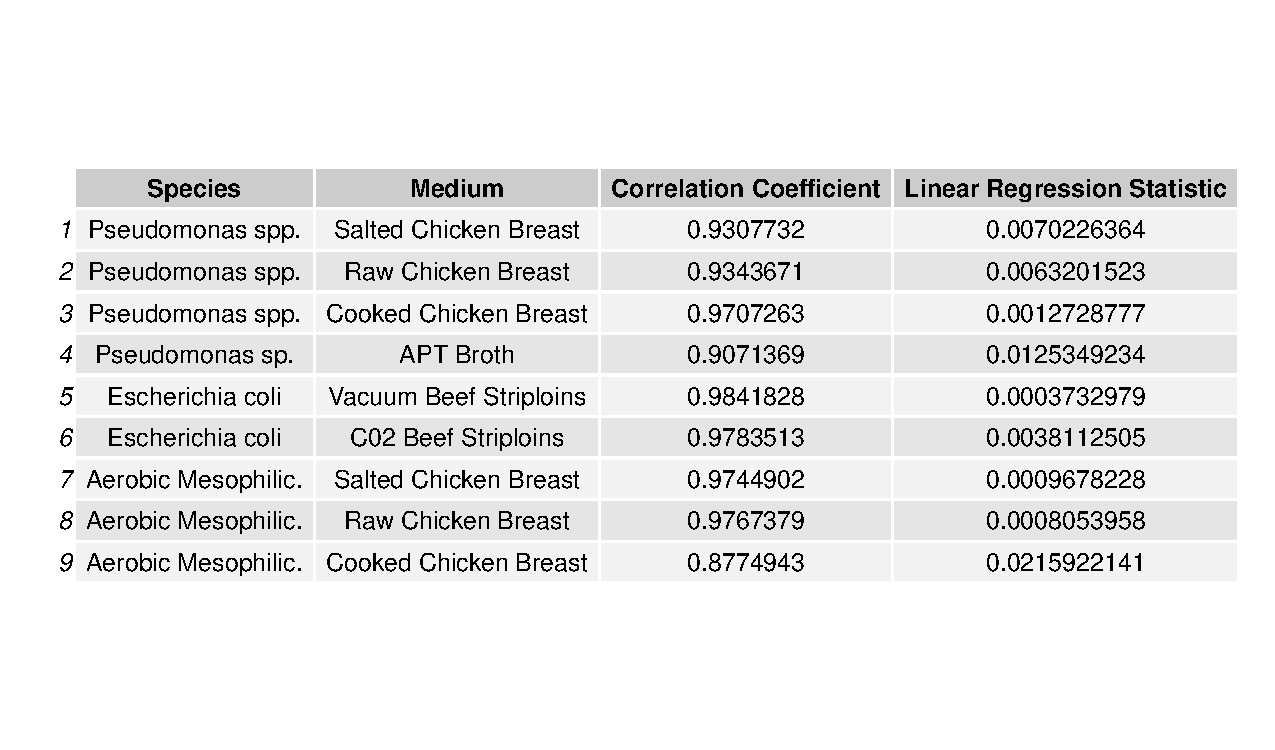
\includegraphics[scale=0.40]{../Results/Temperature_Growthrate.pdf} \caption{Correlation coefficients of square root growth rate and temperature} \label{tab:Correlation Table}
\end{table}
